\textbf{Beschreibung der Datensicht}

\begin{enumerate}
	\item{\textbf{Serversystem}}
	
	Steht für das gesamte bereitgestellte System des Servers, zu dessen Aufgaben Kommunikation mit den Systemnutzern und das Speichern
	von Informationen gehört. Diese Klasse stellt keine Implementierungsklasse dar.
	
	\item{\textbf{Server}}
	
	Stellt ServerSockets für die Clients bereit. Server ist ein Teil der Klasse Serversystem.
	
	\item{\textbf{IPersistence}}
	
	Diese Klasse ist ein Interface und stellt Operationen für Data bereit.
	
	\item{\textbf{Data}}
	
	Über die Klasse Data laufen die eigentlichen Prozesse der Datenspeicherung und Nutzerkommunikation. Es besitzt Methoden, um sowohl User, als auch
	Questions zu speichern oder zu verändern und den Ausgang abgeschlosser Spiele oder Matches zu speichern.
	
	\item{\textbf{Quizapp}}
	
	Ähnlich wie die Klasse Serversystem, ist auch Quizapp keine implementierte Klasse, sondern steht für den ganzen Bereich der App und dessen Nutzer.
	In Quizapp befinden sich die Klassen Client und User und besitzt selbst eine Collection$<$Question$>$ für alle Fragen, damit der Nutzer auch offline, also 
	Serversystemunabhängig spielen kann.
	
	\item{\textbf{Client}}
	
	Die Klasse Client stellt mittels eines ServerSockets eine Verbindung mit dem Serversystem durch die Bereitschaft der Sockets von der Klasse Server her.
	
	\item{\textbf{User}}
	
	In der Klasse User befinden sich alle Informationen über den entsprechenden Nutzer, wie das Serversystem und vielleicht andere Nutzer es registrieren 
	müssen oder wollen. User besitzt unter anderem das Attribut "'role"', wodurch entschieden wird, ob es sich bei dem Nutzer um den Admin oder einen AppNutzer handelt.
	
	\item{\textbf{IGame}}
	
	Diese Klasse ist ein Interface, welches Operationen für die Klasse QuizGame bereitstellt.
	
	\item{\textbf{Quizgame}}
	
	Diese Klasse implementiert IGame und enthält alle Operationen die für den Spiel-, Ein-/Auslog, Registrier- und Updatevorgang von seiten der App
	nötig sind. Daher ist diese Klasse ein Teil von sowohl Spielen, als auch Einloggen/..., beides Assoziationsklassen, welche für die eben genannten Vorgänge
	stehen.
	
	\item{\textbf{Match}}
	
	Die Klasse Match beinhaltet alle Daten, die für den Ablauf eines "1gegen1-Spiels" nötig sind, wie unter anderem die beiden Namen der Spieler, sowie deren momentante Punktzahl usw.
	
	\item{\textbf{Question}}
	
	Diese Klasse beinhalten alle Daten, die für jede Frage benötigt wird, wie ihren Text, ihre Kategorie und zur Auswahl stehenden Antowrten auf die Frage an sich.
	
	\item{\textbf{Spielen}}
	
	Diese Assoziationsklasse steht für den Spielvorgang und benötigt daher die Klassen Question und Match. 
	
	\item{\textbf{Einloggen/Ausloggen/Registrieren/Update}}
	
	Diese Assoziationsklassen steht für die in dessen Namen stehenden Vorgänge und beschreibt damit eine der Relationen von Quizapp und Serversystem.
	
	\item{\textbf{Bearbeiten/Hinzufügen/Löschen}}
	
	Diese Assoziationsklasse beschreibt die Relation der Klasse User in der Rolle des Admin und	Serversystem. Der Admin soll Fragen und Nutzer berarbeiten, löschen 
	oder hinzufügen können.
	
\end{enumerate}

\begin{figure}[H]
	\centering
	\begin{minipage}[t]{\textwidth}
		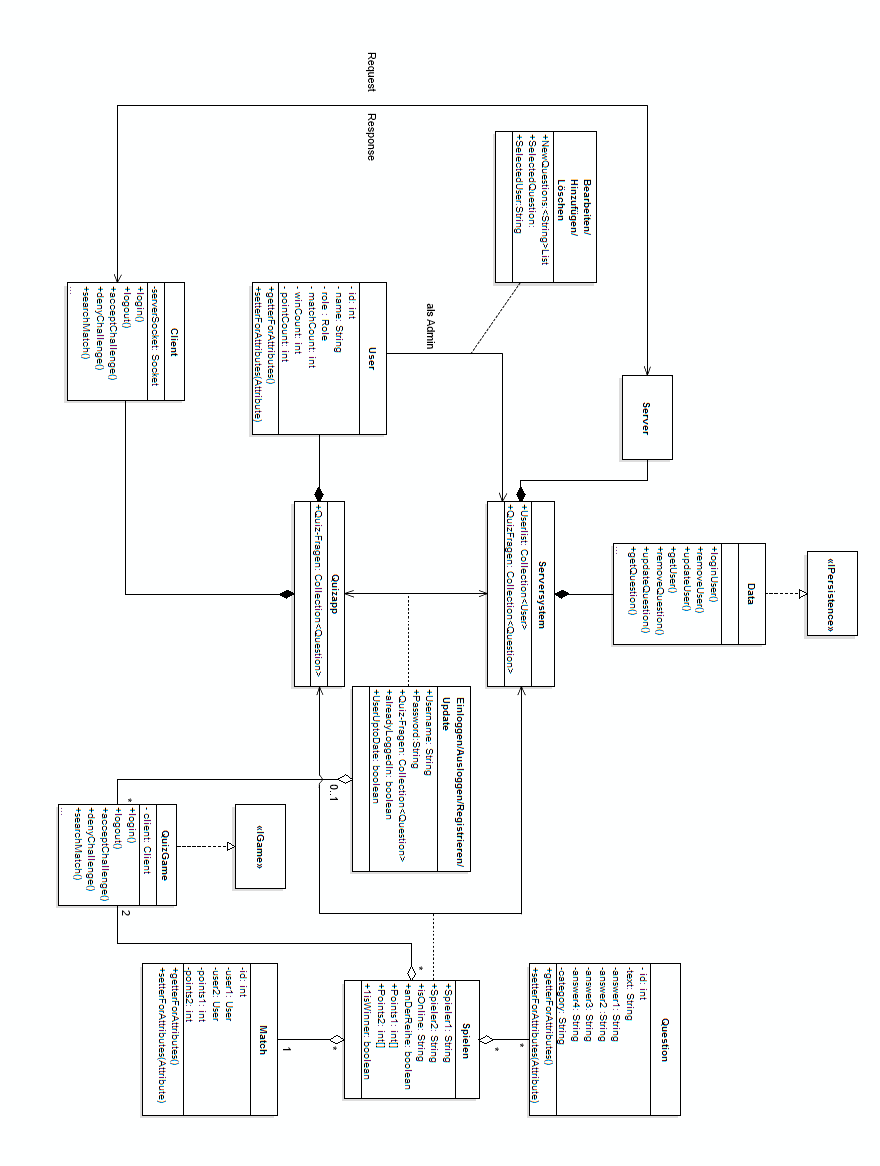
\includegraphics[width=1\textwidth]{Diagramme/DatensichtPaint.png}
		\caption{Datensicht}
		\label{Datensicht}
	\end{minipage}
\end{figure}